\documentclass{article}
\usepackage[english]{babel}
\usepackage[utf8]{inputenc}
\usepackage{johd}
\usepackage{setspace}
\usepackage{fouriernc}
\usepackage{amsmath}

\title{Improving the numerical simulations of glacier flow}

\author{Janine Hay \\
        \small Geography and Planning, University of Saskatchewan, janine.hay@usask.ca\\

}

\date{June 2021} %leave blank
\onehalfspacing
\setlength{\parindent}{0pt}
\setlength{\parskip}{1em}
\begin{document}

\maketitle
\newpage
\tableofcontents
\newpage
testing
\section{Research summary}
Hydrological models are used to simulate changes in the terrestrial component of the water cycle and to predict extreme hydrological events such as floods and droughts. Glaciers, particularly in mountain regions, are a major source of water available during the spring and summer season. Despite the importance of glaciers to the hydrological cycle, they are often not represented correctly in hydrological models. Glaciers are often represented as an "ice cube" model, which only considers the mass balance for a vertical column of the glacier. This type of model does not include glacier dynamics such as flow, ice thickness, and glacier evolution. Proper glacier modelling is essential for understanding the environmental response to a warming climate and remains a major problem in the modelling of Earth System change.  

Modelling of glaciers requires numerical simulations of the glacier dynamics. Glacier dynamics are complex, where a small change in the glacier inputs or equations can cause large changes in the results obtained from glacier models. Numerical simulations of glacier flow are used to describe the movement of the glacier as time passes. A full simulation of glacier flow can be done using the full Stokes equations, which are the most accurate equations available for glacier modelling, but due to their complexity and computational needs, they are unpractical in many circumstances. The shallow ice approximation (SIA) is a method of approximating the full Stokes equation by discarding the small terms.

The goal of this master's research is to investigate glacier modelling processes and create a glacier model modellers can use to simulate the evolution of glaciers. This research will be focused on understanding glacier evolution using numerical simulations of the mass balance and the flow of the glacier. We will be using numerical simulations of glaciers to work towards improving the solving methods for the standard SIA. As a stretch goal, we will be integrating the improved glacier model into the Canadian Hydrological Model (CHM).

This research will help advance the glacier modelling and hydrological modelling fields by creating an improved method of modelling glaciers. 

\newpage
\section{Introduction}
Glaciers are an important part of the hydrological cycle. On a regional scale, glaciers help regulate streamflow, particularly late season streamflow, and contribute to the water available for agriculture, industry, and drinking \citep{Naz2014, Kaser2010, Meier2007}. Warming climates cause glacier melt to increase \citep{Meier2007, Clarke2015, Kaser2010}. Current predictions suggest that Canada will lose between 60\% and 80\% of its glaciers by 2100 \citep{Clarke2015}. On a global scale,  glaciers are the largest contributors to rising sea levels \citep{Marzeion2012}. Approximately 60\% of the rise in sea levels can be contributed to glacier and ice cap melt \citep{Meier2007}.

Modelling of glacier flow is essential for understanding the response of glaciers to climate change. The shallow ice approximation (SIA) is one commonly used method for simulating glacier flow, due to it's ability to be used in large-scale problems without the computational resources that full Stokes equations would require. A known problem with the SIA is that it does not always conserve mass in areas of the glacier where the bed is steep and the ice is thin \citep{Jarosch2013, Hindmarsh1996}. There have been several proposed schemes to address this, such as those introduced by \citet{Jarosch2013, Clarke2015}. These methods, while improvements on the standard solving method, still do not fully solve the mass conservation issue in the SIA. 

The main question to be answered by this research is: How does the numerical method of solving the SIA affects conservation of mass? 

Most large-domain hydrological models do not have a glacier modelling component in them. As such, large-domain hydrological models are not adequate to simulate the impacts of climate change in areas with glaciers. Most large-domain hydrological models, if they include glaciers, model them with a snowmelt model \citep{Pradhananga2020, Naz2014}. These snowmelt models do not accurately account for the unique dynamics of a glacier compared to a general snowpack such as the metamorphosis of snow into firn and then glacier ice, the ice flow dynamics, and the ice melting process \citep{Pradhananga2020}. Conversely, glacier-specific models do not include hydrological processes such as evaporation, transpiration, and canopy interception, making them ineffective at modelling partially glacierized areas \citep{Clarke2015, Maussion2019, Rounce2020}. 

As a stretch goal: How does the inclusion of glacier modelling in large-scale hydrological models affect the model output?



\section{Literature Review}

\subsection{Coupled Glacier Models} 
Even though glaciers are an important part of our hydrological process, they are often not represented in hydrological models. Models such as SUMMA do not explicitly represent glaciers \citep{Clark2015}. To address this gap in the modelling process, coupled glacio-hydrological models are run by modelers to determine the effects of climate change on glaciers and the runoff generated by glaciers \citep{Jost2012, Naz2014}. This coupled glacier model approach helps quantify the contribution of glaciers to streamflow \citep{Jost2012}. The process of incorporating glacier dynamics to the hydrological model is complex because glaciers change in area over time, causing the simulation to need to change the land cover parameter if the model is running over long periods of time \citep{Jost2012}. 

\subsection{Types of Glaciers}
Glaciers can be classified in several different ways. The first is by their shapes; the two main types are valley glaciers and ice cap or ice sheet glaciers. Valley glaciers are long and narrow glaciers that flow in one direction. Valley glaciers that reach water are called tidewater glaciers, and short valley glaciers are called cirque glaciers \citep{Hooke2013}. In valley glaciers, the flow encounters resistance from the valley sides. Much of the movement in valley glaciers is due to sliding at the bed of the glacier \citep{Nye1952}. Ice cap glaciers are glaciers that spread out from a central dome in all directions. There is overlap between the two glaciers; often ice cap glaciers will feed outlet glaciers, which are glaciers that act like valley glaciers but are fed by an ice cap.

The other way to categorize glaciers is by their thermal characteristics: polar glaciers, polythermal glaciers, and isothermal glaciers. Firstly, polar glaciers are glaciers where the ice temperature is below the melting point all over the glacier, with the possible exception of the glacier bed \citep{Hooke2013}. The glacier bed may be above freezing because of the ground energy flux from the earth. Due to the ground energy flux, polar glaciers can either be frozen or unfrozen from their beds \citep{Hooke2013}. Secondly, polythermal glaciers are glaciers where some of the ice is below the melting point, and some of the ice is at the melting point \citep{Hooke2013}. Thirdly, isothermal glaciers are glaciers where all ice in the glacier is at the melting temperature \citep{Hooke2013}. The melting temperature is not always defined as 0C though. This is because of the water content in the ice and the pressure of the glacier \citep{Lliboutry1976}. \citet{Lliboutry1976} showed that depending on the substances dissolved in water, melt temperature can fluctuate a couple hundredths of a degree. For an isothermal glacier to slide on its bed, the interface between the rock and the bed of the glacier must reach the melting point \citep{Lliboutry1976}. The glacier then slides over the bed using the melted water as a lubricating medium between the bed and glacier ice \citep{Fowler1979}. 

\subsection{Mass Balance}
Glaciers form in areas where the accumulation of the snow over the winter exceeds the melt rate of the glacier in the spring and summer \citep{Hooke2013}. The snow from the glacier that stays for more than a year goes through snow metamorphism and is called firn. After several years the firn will turn to solid ice \citep{Hooke2013}. As this glacier ice flows, it moves into the ablation area of the glacier, where the melt exceeds the snow fall of the glacier. Thus, the mass balance of the glacier at a given point is defined as 
\begin{equation}
    \frac{dS}{dt} = A - M
\end{equation}
where $S$ is the storage of ice in the glacier, $A$ is the accumulation of the glacier, and $M$ is the ablation of the glacier. Accumulation is found using 
\begin{equation}\label{Accumulation}
A = \frac{\rho_{water}}{\rho_{ice}}f_{snow}P
\end{equation}
where $\rho_{water}$ is the densities of water, $\rho_{snow}$ is the density of ice, and $P$ is the total amount of precipitation. $f_{snow}$ is the fraction of total precipitation that falls as snow \citep{Jarosch2013}.

Glacier mass balance models can be classified into two different types, temperature-index models and energy-balance models \citep{Hock2005}. Temperature-index models rely on an empirical relationship between the air temperature and the amount of melt while energy balance models attempt to quantify the melt as part of the heat-balance equation \citep{Hock2003}. Temperature-index models are widely used because of their low data requirements, relative ease in interpolating air temperatures for forecasting, and they are computationally simple \citep{Hock2003}. The most basic version of the temperature index model is the degree day version such as the one used in \citet{Clarke2015} regional glacier model (RGM). Temperature-index models group all factors of surface-energy balance into a proportionality coefficient, which is used to calculate net melt with air temperature \citep{Pradhananga2020}. This assumes that air temperature is the main contributing factor of melt. The extended temperature index model, such as the one used by \citet{Marzeion2012}, is the response to getting more realistic versions of the temperature melt model, without giving up the computational advantages of the melt model. Temperature-index models perform well on a seasonal level over catchments, but if daily melt rates are required an energy balance model is required \citep{Gudmundsson2009, Hock2003}. This is because even though other sources of melt energy, such as radiation, are often more directly responsible for melt \citep{Pradhananga2020}. 


Temperature-index mass balance modelling use air temperature as the main factor controlling the melt of a glacier \citep{Pradhananga2020}. The equations are relatively easy to implement and require limited data, for the most basic of them just temperature and precipitation data is required \citep{Clarke2015}. While comparisons of temperature-index models with energy balance models have shown that the performance of temperature-index models often matches energy balance performance \citep{Hock2005}, especially for seasonal performance \citep{Gudmundsson2009}. Methods for solving this mass balance are generally relating the amount of ablation to the degree day factor, a proportionality coefficient to calculate the melt based on air temperature, of the glacier\citep{Pradhananga2020}. The basic temperature-index model looks at the ablation and accumulation of a glacier to calculate the mass balance. Ablation can be found with

\begin{equation} \label{Melt}
M = f_{dd}D
\end{equation}

where D is the number of positive degree days and $f_{dd}$ is the degree day factor. $f_{dd}$ can either be held constant in time, or extended to show a dependence on radiation
\begin{equation}
f_{dd} = f_m+ a_{snow/ice}I
\end{equation}
 where $f_m$ is the bulk melt factor, $a_{snow/ice}$ is the radiation factor, and I is the direct solar radiation \citep{Clarke2015}. 

Energy-balance models, equation \ref{energybalance} assess the energy at the surface of the glacier to determine melt \citep{Hock2005}. 
\begin{equation}\label{energybalance}
Q_M = Q_n+Q_h+Q_e+Q_p+Q_g-\frac{dU}{dt}
\end{equation}
where $Q_n$ is the net radiation, $Q_h$ is the sensible hear, $Q_e$ is the latent heat, $Q_g$ is the ground energy flux, $Q_p$ is the energy supplied by rain, $\frac{dU}{dt}$ is the change in internal energy, and the energy consumed by melt is $Q_M$ \citep{Hock2005, Hooke2013}.  Collecting the complete energy budget fluxes directly is seldom available for an individual glacier, and even rarer for long periods of time, because of the equipment requirements. However, estimations of the terms in an energy budget are available \citep{Hock2005}. Energy-balance models are necessary on glaciers where the daily temperature does not vary greatly throughout the year, such as tropical glaciers \citep{Sicart2008}. On glaciers such as these, the dominant contributing flux to the melt is shortwave radiation \citep{Pradhananga2020, Sicart2008}.

\subsection{Glacier Flow}
We treat ice in glaciers as a fluid and model the flow of the glacier using computational fluid dynamics. The large scale computational fluid dynamics are similar to modelling the ocean or the atmosphere, except that instead of examining factors such as turbulence or the Coriolis force, for glaciers, we evaluate the glacier dynamics such as the ablation, accumulation, and flow of ice. Glacier flow is modeled in numerious ways, the most physically accurate way being the full Stokes model, and the most common in large-scale models being the shallow ice approximation (SIA). The full Stokes model is not used over large domains and over long time periods because of the substantial computational resources required to run the model on a paleo time scale or over large domains. The computational power required makes the inclusion of full Stokes models in large-scale models complicated and leaves a place in the modelling community for the continued improvement of the SIA. The SIA is one method of approximating the flow of the glacier. The SIA scales the small scale terms in Stokes model so that they can be expressed as a power series \citep{Kirchner2016, Emmanuel2004}. The SIA is only appropriate for modelling bulk ice flow, and should not be used for modelling small-scale dynamics such as surface velocity, ice streams,  and ice domes \citep{AHLKRONA2016,LEMEUR2004}.

\subsubsection{Stokes Model}
The full Stokes model is a differential equation model that includes all ice dynamic flow terms. The linear momentum is described by
\begin{subequations}\label{Stokes}
\begin{gather}
    \frac{\partial \tau_{xx}}{\partial x} + \frac{\partial \tau_{xy}}{\partial y}+ \frac{\partial \tau_{xz}}{\partial z} = 0\\
    \frac{\partial \tau_{xy}}{\partial x} + \frac{\partial \tau_{yy}}{\partial y}+ \frac{\partial \tau_{yz}}{\partial z} = 0\\
    \frac{\partial \tau_{xz}}{\partial x} + \frac{\partial \tau_{yz}}{\partial y}+ \frac{\partial \tau_{zz}}{\partial z} = \rho g
\end{gather}
\end{subequations}
where $\tau_{ij}$ is the stress tensor, $\rho$ is the density of ice, and $g$ is acceleration due to gravity \citep{LEMEUR2004}.The full Stokes model also includes the mass conservation equation \citep{LEMEUR2004}. The stress tensor can then be written with
\begin{equation}
    \tau_{ij} = \tau_{ij}' + \rho \delta_{ij}
\end{equation}
where $\tau_{ij}'$ is the deviatoric stress tensor and $\rho\delta_{ij}$ is the isotropic pressure \citep{LEMEUR2004, soucek2008}. $\delta_{ij}$ is the Kroneker symbol \cite{LEMEUR2004}. Assuming that the ice is incompressible and that the density is homogenous the ice velocity equation can be written as

\begin{equation} \label{mass conservation}
\frac{\partial v_x}{\partial x} + \frac{\partial v_y}{\partial y}  +\frac{\partial v_z}{\partial z} =0   
\end{equation}

where $v_x$, $v_y$, and $v_z$ are the corresponding $x$,$y$, and $z$ components of the glacier velocity \citep{LEMEUR2004,soucek2008}. Glaciers are bound by the free surface and the bed of the glacier leading to the free surface boundary condition of 
\begin{equation}\label{free surface}
\frac{\partial s}{\partial t} + v_x \frac{\partial s}{\partial x}+ v_y \frac{\partial s}{\partial y} -v_z = m_s
\end{equation}
where $s$ and is the representation of the free surface, and $m_s$ is the mass balance at the surface \citep{LEMEUR2004, Greve2009}. As well as the bed surface boundary condition is
\begin{equation}\label{bed}
\frac{\partial b}{\partial t} + v_x \frac{\partial b}{\partial x}+ v_y \frac{\partial b}{\partial y} -v_z = m_b
\end{equation}
where $b$ and is the representation of the free surface, and $m_b$ is the mass balance at the bed \citep{LEMEUR2004, Greve2009}.
\subsubsection{Shallow ice approximation}
The assumptions made in the SIA are that the ice is shallow and that vertical shearing dominates horizontal sliding. To calculate the ice thickness for the SIA equation \ref{mass conservation} is combined with the free surface boundary condition equation \ref{free surface}, and the bed boundary condition equation \ref{bed}\citep{LEMEUR2004, Greve2009}. First equation \ref{mass conservation} x and y terms are integrated from the glacier bed to the ice surface using Leibniz's rule
\begin{subequations} \label{xandy}
\begin{gather}
    \frac{\partial}{\partial x}\int_b^s v_x dz = \int_b^s \frac{\partial v_x}{\partial x}dz+v_x|_{z=s}\frac{\partial s}{\partial x}-v_x|_{z=b}\frac{\partial b}{\partial x} \\
    \frac{\partial}{\partial y}\int_b^s v_y dz = \int_b^s \frac{\partial v_y}{\partial y}dz+v_y|_{z=s}\frac{\partial s}{\partial y}-v_y|_{z=b}\frac{\partial b}{\partial y}
\end{gather}
\end{subequations}
and the z term is simply
\begin{equation}\label{z}
    \int_b^h\frac{\partial}{\partial z}dz = v_z|_{z=s}-v_z|_{z=b}
\end{equation}
When equations \ref{xandy} and \ref{z} are plugged into equation \ref{mass conservation} it becomes
\begin{equation}
    \int_b^s \frac{\partial v_x}{\partial x}dz+v_x|_{z=s}\frac{\partial s}{\partial x}-v_x|_{z=b}\frac{\partial b}{\partial x}+\int_b^s \frac{\partial v_y}{\partial y}dz+v_y|_{z=s}\frac{\partial s}{\partial y}-v_y|_{z=b}\frac{\partial b}{\partial y}+v_z|_{z=s}-v_z|_{z=b} = 0
\end{equation}
The free surface (equation \ref{free surface}) and bed (equation \ref{bed}) boundary conditions of the glacier are then applied to yield
\begin{equation}
    \int_b^s \frac{\partial v_x}{\partial x}dz+\int_b^s \frac{\partial v_y}{\partial y}dz+ \frac{\partial s}{\partial t}-\frac{\partial b}{\partial t} -m_s+m_b = 0
\end{equation}
We then introduce the flux $q$ to represent the volume of ice flow and the vertically integrated horizontal velocities. We assume that their is no melting at the bed, so $m_s-m_b=m$ and we substitute in $h = s-b$ to obtain
\begin{equation}\label{ice thickness}
\frac{\partial h}{\partial t} + \nabla \cdot q = m
\end{equation}


where $q$ is the flux of the glacier , $h$ is the thickness of the glacier ice, and $m$ is the mass balance of the glacier \citep{Jarosch2013,Greve2009}.
\subsubsection{Solving the shallow ice approximation}
The widely used method for solving the SIA is to treat equation \ref{ice thickness} as a diffusion problem, where 
\begin{equation} \label{diffusion1}
    q= D(\nabla h + \nabla b)
\end{equation}
where D is the diffusion coefficient \cite{Jarosch2013}. The method then applies an explicit time stepping method to update the ice surface elevation

\begin{equation} \label{timestep}
\frac{\tilde{h}^{i+1}-h^i}{\Delta t} - \nabla \cdot (D^i (\nabla h^{i} + \nabla b^{i})) = m^i
\end{equation}
The ice thickness is then clipped using equation \ref{clip}, which takes any negative values of ice thickness and sets them back to 0. 
\begin{equation}\label{clip}
h^{i+1}=max(\tilde{h}^{i+1},0)
\end{equation}
There are two common methods used for discretization in ice sheet models, M1 and M2. Both use a regular mesh with a finite volume discretization \cite{Jarosch2013,Hindmarsh1996,Huybrechts1996}.  Each cell in the mesh has a x and y flux value. The x flux value of $q^x_{k, l+1/2}$  is at the cell boundary between the $(k,l)$ and $(k+1,l) $ cells and the y flux value of $q^y_{k+1/2, l}$ is at the cell boundary between the $(k,l)$ and $(k,l+1)$ cells, see Figure \ref{fig:Grid}. 
\begin{figure}[H]
    \centering
    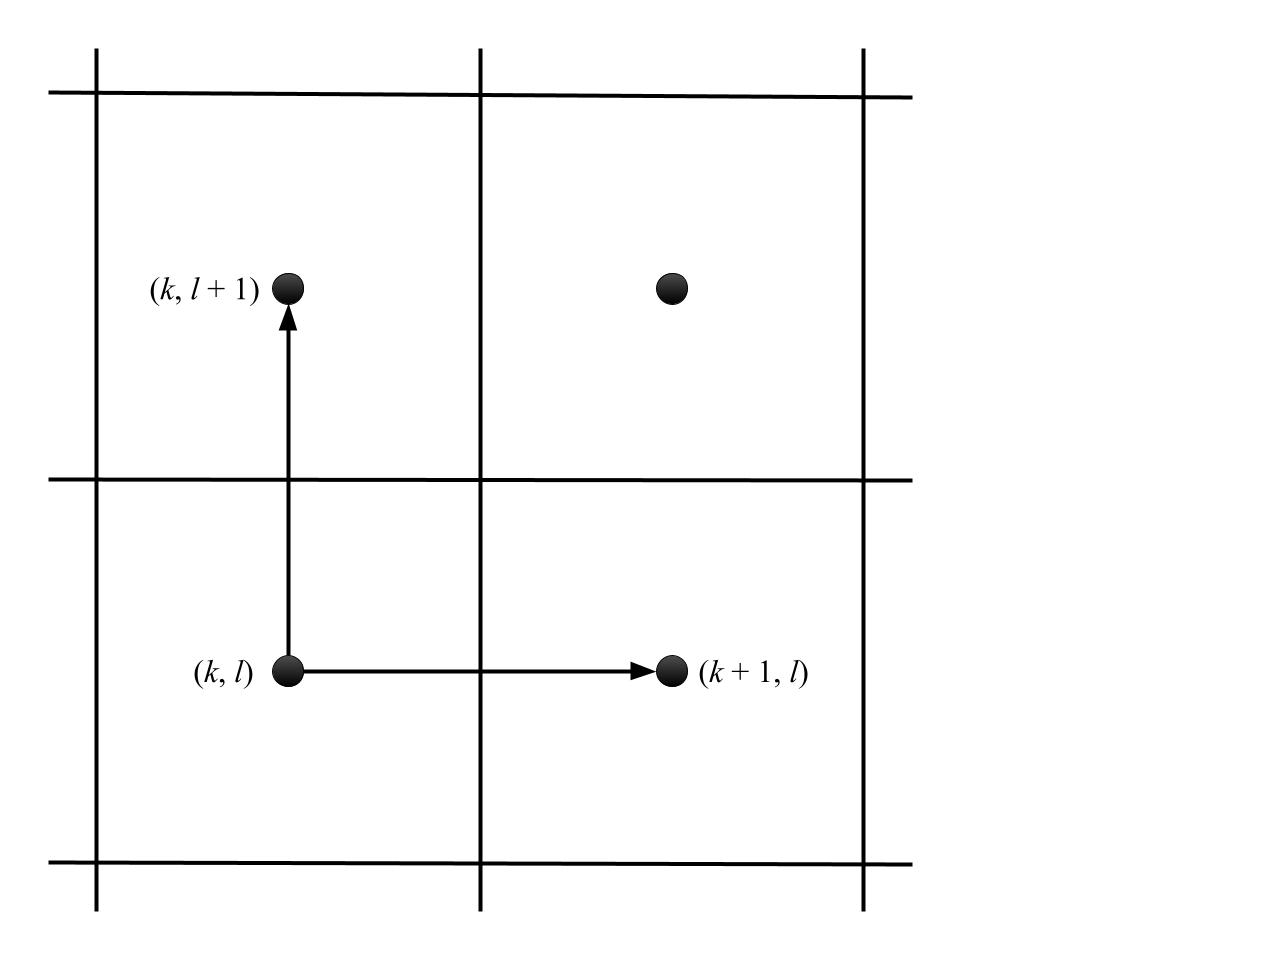
\includegraphics[width=10cm]{Grid.jpg}
    \caption{Visual depiction of the mesh}
    \label{fig:Grid}
\end{figure}
M1 and M2 relate the fluxes the the surface elevation differences with
\begin{subequations}
\begin{gather}
    q^{y, i+1}_{k, l+1/2}=-D^i_{k, l+1/2}\frac{\tilde{s}^{i+1}_{k, l+1}-(\tilde{s}^{i+1}_{k, l}}{\Delta y} \\
    q^{x, i+1}_{k+1/2, l}=-D^i_{k+1/2, l}\frac{\tilde{s}^{i+1}_{k+1, l}-\tilde{s}^{i+1}_{k, l}}{\Delta x}
\end{gather}
\end{subequations}
The norm of the surface gradient at the cell boundary is then defined to be 
\begin{equation}
    |\nabla s ^i|^{n-1}_{k+1/2,l} = \left[\left( \frac{s^i_{k,l+1}-s^i_{k,l-1}+s^i_{k+1,l-1}}{4\Delta y}\right)^2+\left( \frac{s^i_{k+1,l}-s^i_{k,l}}{\Delta x}\right)^2 \right]^{\frac{n-1}{2}}
\end{equation}


The M1 discritization used the average value of $h$ over the cell
\begin{equation}
    D^i_{k+1/2,l}=\Gamma\left(\frac{h^i_{k,l}+h^i_{k+1,l}}{2}\right)^{n+2}|\nabla s ^i|^{n-1}_{k+1/2,l}
\end{equation}
and the M2 discritization is the average over $h^{n+2}$
\begin{equation}
    D^i_{k+1/2,l}=\Gamma\left(\frac{{h^i_{k,l}}^{n+2}+{h^i_{k+1,l}}^{n+2}}{2}\right)|\nabla s ^i|^{n-1}_{k+1/2,l}
\end{equation}
where $\Gamma$ is a proportionality coefficient relative the stress of the ice \citep{Jarosch2013}. 

The problem with the above method is that the spatial discretizations used to solve for the diffusion equations (equation \ref{diffusion1}) do not preserve positivity in specific scenarios, such as u-shaped valleys, leading to negative ice thickness values when the terrain is steep and the ice is thin. When this happens, equation \ref{clip} sets the value back to zero, violating conservation of mass \citep{Jarosch2013, Hindmarsh1996}. The easiest way to demonstrate this is by rewriting the ice thickness equation \ref{ice thickness} as
\begin{equation}\label{hypero}
\frac{\partial h}{\partial t} - \nabla \cdot \left( \Gamma h^{n+2} |\nabla(b+h)|^{n-1}\nabla(b+h)\right) =m
\end{equation}
when the bed slope is small or the ice is thick the  $\nabla(b+h)$ term is dominated by the ice thickness and equation \ref{hypero} is parabolic, and so discretizations schemes designed for parabolic terrain will preserve the positivity of our ice thickness \cite{Jarosch2013}. In steep bed terrain or when the ice is this, the $\nabla(b+h)$ term is dominated by the bed slope, making equation \ref{hypero} hyperbolic \cite{Jarosch2013}. The discretization schemes used in a parabolic scenario may than produce negative ice thickness values.



\subsubsection{Glen's flow law flux}
Glen's flow law is one method used to determine the relationship between the stress and strain of the ice  \citep{AHLKRONA2016}. Glen's flow law is defined as
\begin{equation}\label{Glen}
\epsilon_e = A \sigma^n_e
\end{equation}
where $A$ is Glen’s flow law rate factor, $n$ is Glen’s flow law power law constant and is equal to 3, $\epsilon_e$ is strain rate, and $\sigma_e$ is the applied stress \citep{Hooke2013, Nye1952}. \citep{Jarosch2013, AHLKRONA2016}.

With the assumptions from SIA, the relative components of the shear stress are $\tau_{xz}$ and $\tau_{yz}$. All other components of the stress are considered negligible \citep{Greve2009}. This simplifies equation \ref{Stokes} to 
\begin{subequations}\label{horSIA}
\begin{gather}
    \frac{\partial \tau_{xz}}{\partial z} = \rho g \frac{\partial s}{\partial x} \\
    \frac{\partial \tau_{yz}}{\partial z} = \rho g \frac{\partial s}{\partial y}
\end{gather}
\end{subequations}
which can be integrated to
\begin{subequations}\label{horSIAint}
\begin{gather}
    \tau_{xz} = -\rho g(s-z) \frac{\partial s}{\partial x} \\
    \tau_{yz} = -\rho g(s-z) \frac{\partial s}{\partial y}
\end{gather}
\end{subequations}
since the right hand side does not depend on $z$ \citep{Greve2009}. The applied stress of the ice is then
\begin{align}
    \sigma_e &= \sqrt{\tau^2_{xz}+\tau^2_{yz}} \nonumber\\
     &= \rho g(s-z) |\nabla s| 
\end{align}
This result is then inserted into equation \ref{Glen} as the the applied stress \citep{Greve2009}. 
\begin{subequations}

\begin{gather}
   \frac{1}{2} \left(\frac{\partial v_x}{\partial z}+\frac{\partial v_z}{\partial x}\right) = -A[\rho g (s-z)]^n|\nabla s |^{n-1}\frac{\partial s}{\partial x} \\
    \frac{1}{2} \left(\frac{\partial v_y}{\partial z}+\frac{\partial v_z}{\partial y}\right)  = -A[\rho g (s-z)]^n|\nabla s |^{n-1}\frac{\partial s}{\partial y} 
\end{gather}
\end{subequations}


Based on the order of magnitude, we can neglect the horizontal derivatives of the vertical velocity so that
\begin{subequations}
\begin{gather}
    \frac{\partial v_x}{\partial z} = -2A[\rho g (s-z)]^n|\nabla s |^{n-1}\frac{\partial s}{\partial x} \\
    \frac{\partial v_y}{\partial z} = -2A[\rho g (s-z)]^n|\nabla s |^{n-1}\frac{\partial s}{\partial y} 
\end{gather}
\end{subequations}
which can be integrated from the bed height to the free surface of the glacier in order to calculate our flux $q$
\begin{subequations}
\begin{gather}\label{q}
    q = -\Gamma  h^{n+2} |\nabla h+\nabla b|^{n-1} (\nabla h + \nabla b)  \\
    \Gamma = \frac{2A (\rho g)^n}{n+2} 
\end{gather}
\end{subequations}
giving us the flux method used in the standard solving method of the SIA \citep{Jarosch2013, Greve2009}.


\subsubsection{MUSCL flux method}
A mass conserving solution, called the MUSCL superbee method from here on, was proposed by \citet{Jarosch2013} as a possible solution to address the violation of conservation of mass caused by the stand solving method for the SIA. This method addresses the root of the conservation problem, the calculation of $D$, the diffusion coefficient. To do this, the second-order Monotone Upstream-centered Schemes for Conservation Laws (MUSCL) were modified for SIA. This flux limiter modifies the ice flux to be 
\begin{subequations}\label{fluxlimiter}
\begin{gather}
q  = \omega h^{n+2}  \\
\omega  = \Gamma | \nabla h + \nabla b |^{n-1}(\nabla h + \nabla b) 
\end{gather}
\end{subequations}

The flux, $q$, is replaced in equation \ref{ice thickness} with equation \ref{fluxlimiter}, creating

\begin{equation}\label{jarosch}
\frac{\partial h}{\partial t} + \nabla \cdot (\omega h^{n+2}) = m 
\end{equation}
This flux limiter scheme is positive preserving when equation \ref{jarosch} becomes hyperbolic, and improves conservation of mass in areas where the ice is thin and the terrain is steep \citep{Jarosch2013}. 
\begin{figure}[H]
    \centering
    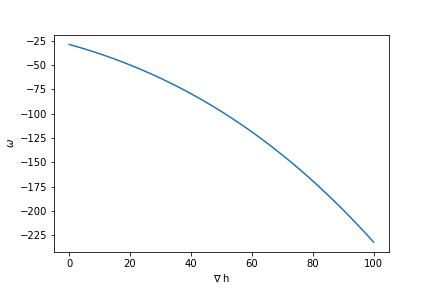
\includegraphics[width=13cm]{Iceflux.png}
    \caption{plot of $\omega$ verses $\nabla h$, for a clearer idea of the effects of equation \ref{fluxlimiter}
}
    \label{fig:Iceflux}
\end{figure}
\begin{figure}[H]
    \centering
    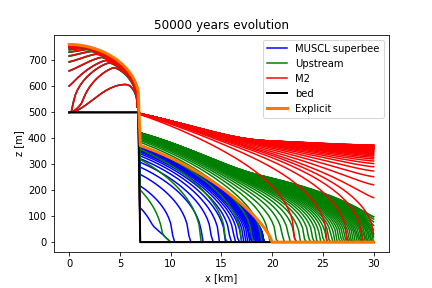
\includegraphics[width=13cm]{JaroschPaperFigure3.png}
    \caption{A reproduction of a figure from \citet{Jarosch2013} showing the results of various models applied to a cliff benchmark. Upstream is solving the SIA by applying an upwinding scheme to it. M2 is the results from the standard numerical solving method described in equation \ref{timestep}. Eqs (56) and (57) are the exact solutions to this glacier bed. Each line is a 1000 year timestep over 50 000 years. From this you can see, that the Upstream and M2 method do not converge towards the explicit solution, and have extra mass, the MUSCL superbee method does converge towards the exact solution.
}
    \label{fig:JaroschPaper}
\end{figure}

The MUSCL superbee method was attempted to be adapted for more complex topography by \citet{Clarke2015}, who found that when adapting the diffusivity constants to their model, they still found violations of conservation of mass occasionally. Their solution to this was to check for conservation violations at every timestep, and if one was found, apply an adaptive time step and recalculate the ice thickness. 



\subsection{Research Gaps}
Many of the models based on the SIA have research gaps. The one being addressed in this research is the violation of mass conservation that arises from current methods of solving the SIA. The standard method does not conserve mass in in steep terrain where the bed is thin due to the spatial discretization. The the MUSCL superbee method proposed by \citet{Jarosch2013} is not applicable to glaciers with complex topography or glaciers with multiple flow lines, as is discussed in \citet{Maussion2019}. This means that it is not applicable in many real world applications currently, and only works as a benchmark to judge your results against. There are also new numerical solving methods for these types of conservation problems, called conservative methods for finite difference methods associated with hyperbolic equations, which may work to better model glaciers when using the SIA. 




\section{Research Design}

The proposed research is on applying numerical methods to glacier models. The research starts by reproducing the results from the \citet{Jarosch2013} paper. For this, first a basic mass balance model needs to be set up. This mass balance model can then be used to implement the SIA. By reproducing these results, we are setting up the basis to be able to expand a mass conservation solution to the shallow ice-approximation into more complex glacier topology. A method of addressing this is may be expanding on the method for conserving mass balance presented in \citet{Jarosch2013} paper so that it can be applied to varying glacier beds and flow lines. Another method may be by using a different numerical solver method for the shallow ice model.
\subsection{Model creation}
To implement this research, the first step is to reproduce the results from the standard method and \citet{Jarosch2013} mass conserving method. Then, a different numerical method will be implemented for the SIA that will address the need for mass conservation in the SIA. The first step in this process was identifying the glacier modeling equations that will be used. The second step is looking at state-of-the-art numerical techniques that can be applied to the standard ice approximation. One of these methods must then be applied to the glacier modeling equations and write up the model so that it can be forced with mass balance data.
\subsection{Synthetic data}
For model validation, the model will first be run with synthetic data. The model results will be compared against the mass conserving method done by \citet{Jarosch2013} the exact solutions from \citet{Bueler2005}, and the standard solving method described in \citet{Jarosch2013, Hindmarsh1996}. For this section there will be no data requirements, the SIA will be forced with synthetic mass balance data for the cliff benchmark. 
\subsection{Realistic data}
The third part of this research will be running the model over various glacier basins using the mass balance models produced by either the Cold Regions Hydrological model (CHRM) or the Structure for Unifying Multiple modelling Alternatives (SUMMA). 

\subsubsection{Study area}
The first two study areas that will be looked at are Peyto Glacier and Athabasca Glacier. The Peyto glacier is a mountain outlet glacier from the Waputik ice field. It is one of the glaciers currently being monitored by the University of Saskatchewan.It was first surveyed in 1933. Mass balance data has been been collected since 1965 and is available though \citet{WGMS2020}. The Athabasca glacier is an outlet glacier of the Columbia ice field. It is also currently being monitored by the University of Saskatchewan. It was first surveyed in 1945. Mass balance data has been collected since 1980 and is available through \citet{WGMS2020}.


\subsection{Stretch goal}
The final stretch goal for this research is to incorporate the improved glacier model into the CHM modelling framework, and using that implementation to evaluate how the addition of glacier dynamics into the CHM modelling framework affects water availability predictions. 


\section{Scholarly and Societal Relevance}
The scholarly and societal relevance in this research is in evaluating how new numerical methods affect mass conservation in a glacier model using the SIA. This evaluation will take into account the performance of the model at the cliff benchmark, as well as over various isothermal mountain glaciers. Addressing this will improve models of the glacier dynamics and lead to better descriptions of how climate effects the water available from glaciers and glacier evolution. 

\section{Constraints}
Most of the constrains in the research are overcoming technical barriers and overcoming impacts of COVID-19 on the working environment and ability to collaborate.

For technical barriers, modelling of glaciers requires a large amount of computational power, both for the complexity of the calculations and the timescales needed to be run over. To address this, we have access to high performance computing facilities such as Plato.  

Another technical barrier is the access to glacier data, since it is notoriously difficult to have consistent glacier data. There are multiple groups now that have gathered global databases of glacier data. Included in these is the World Glacier Monitoring Service, which has data on the balance, length, volume, and area of glaciers, and the Randolph Glacier Inventory \citep{RGI2017}, which has outlines of glaciers.

COVID-19 has caused impacts on how we work and our working environments. The main challenges with this are adjusting to different working situations, which just takes time to adjust for, and communicating with others in a remote setting. The available technology makes this feasibly and allows you to work physically separated from others while still being able to work with them.

\section{Dissemination}
This research will be disseminated through scientific papers and conferences. The thesis will be written as a final product and published through the university.

The results from the research will be written up in several peer-reviewed scientific papers.

Presentation of this research will likely be at the American Geophysical Union (AGU) and possibly the European Geophysical Union (EGU) based on my planned time for the completion of major steps in my research. It is likely that the presentation of research at these events will be through the form of poster presentations and in-person conversations.

\section{Budget}
There is not expected to be a large amount of overhead in costs, since there is no required field work for the thesis. Most costs will come from conference travel costs and publishing costs for each paper. 

\begin{table}[h]
    \centering
    \begin{tabular}{lll}
    Conference
         &  \$3000 per conference\\
         & up to two conferences \\
    Publishing costs
        & \$ 2000 per a paper \\
        & 1-2 papers \\
    
    \end{tabular}
    \caption{Budget for Master's Thesis}
    \label{tab:my_label}
\end{table}

\section{Timeline}
This masters will be completed over a 2 year period, starting in September 2020, and finishing by September 2022. A tentative plan is laided out below in Figure \ref{fig:Timeline}

\begin{figure}[H]
    \centering
    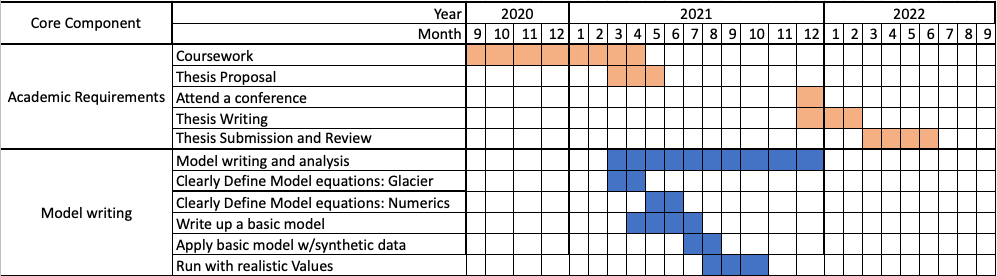
\includegraphics[width=16cm]{GahnttChart.png}
    \caption{}
    \label{fig:Timeline}
\end{figure}

\bibliographystyle{johd}
\bibliography{bib}


\end{document}